% Chapter Template

\chapter{FDTD - Three-Dimensional Scenario} % Main chapter title

\label{Chapter4} % Change X to a consecutive number; for referencing this chapter elsewhere, use \ref{ChapterX}

%----------------------------------------------------------------------------------------
%	SECTION 1
%----------------------------------------------------------------------------------------

For the three-dimensional scenario, we will see a lot of similarities with the previous versions. The methodology is again pretty much the same. It might seem a bit intimidating at first, when considering that the number of vector components we need to deal with has doubled. This scenario is also where optimization really matters, as we are dealing with $N^3$ amounts of data. Nonetheless, if we focus on just the most basic implementation, taking this step by step, and splitting the effort into small parts, we can easily move forward.

\clearpage

\section{3D Discretization}

The easiest way to explain the 3D discretization is with Figure \ref{fig:fdtd3dDisc}.

\begin{figure}[h!]
	\centering
	\includegraphics[scale=0.6]{Figures/fdtd3dDisc}
	\decoRule
	\caption[3D Electric Discretization]{The figure shows the vectors for the electric field, with the respective magnetic vectors.}
	\label{fig:fdtd3dDisc}
\end{figure}

As seen previously, the magnetic field is staggered in every axis by half the step size. The figure also gives a hint as to how the vector components are laid out in our domain. If we were to take only the electric field into the consideration, we can show where each electric vector belongs (Figure \ref{fig:fdtd3dFull}). 

\begin{figure}[h!]
	\centering
	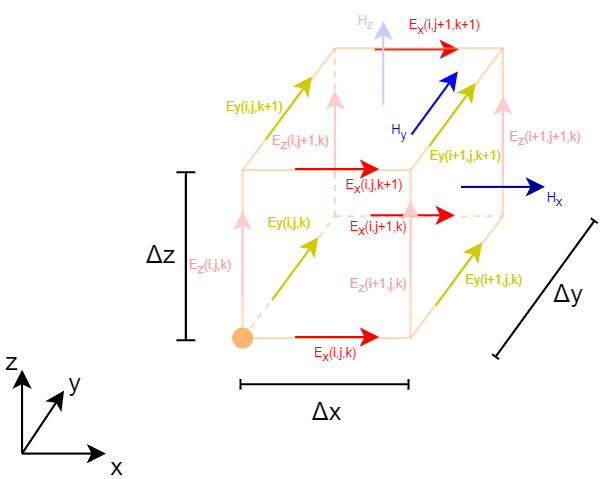
\includegraphics[scale=0.6]{Figures/fdtd3dFull}
	\decoRule
	\caption[3D Electric Discretization]{The figure shows the vectors for the electric field, with the respective magnetic vectors.}
	\label{fig:fdtd3dFull}
\end{figure}

Despite the fact that the image above is fairly cluttered with information, we only need to use bits of it at a time. We will notice in the next section that the electromagnetic curls for the three-dimensional scenario can be derived in the same way that we used for the two-dimensional scenario.

%-----------------------------------
%	SUBSECTION 1
%-----------------------------------
\subsection{3D Electromagnetic Curls}

In the previous chapter, we derived the vector curl for $H_z$ and from there arrived at the update equation. Luckily the curl is exactly the same in the three-dimensional scenario, however we must revise our formula to account for the added dimension, starting by changing the indexing scheme to the following:

\begin{equation}
	\label{eqn:indexing3DElectric}
	E_{i,j,k} = E(i \cdot \Delta x , j \cdot \Delta y, k \cdot \Delta z)
\end{equation}

From there, we repeat the same process as before.
\begin{multline}
	\label{eqn:3dHzCurl1}
	\oint \vec{E} \cdot d\vec{s} = - \frac{d}{dt} \iint \mu \cdot \vec{H} \cdot d\vec{A} \\
	\Rightarrow E_x(i,j,k) \cdot \Delta x - E_x(i,j+1,k) \cdot \Delta x + E_y(i+1,j,k) \cdot \Delta y - E_y(i,j,k) \cdot \Delta y \\ = -\frac{d}{dt}(\mu \cdot H_z(i,j,k) \cdot \Delta x \cdot \Delta y)
\end{multline}

\begin{equation}
	\label{eqn:3dHzCurl2}
	\frac{d}{dt} H_z(i,j,k) = -\frac{1}{\mu} \cdot (\frac{E_x(i,j,k) - E_x(i,j+1,k)}{\Delta y} + \frac{E_y(i+1,j,k)- E_y(i,j,k)}{\Delta x})
\end{equation}

Using a uniform mesh size again, $\Delta x = \Delta y =  \Delta z = \Delta s$, we can simplify equation \ref{eqn:3dHzCurl2} to:

\begin{equation}
	\label{eqn:3dHzCurl3}
	\frac{d}{dt} H_z(i,j,k) = -\frac{1}{\mu \cdot \Delta s} \cdot ((E_x(i,j,k) - E_x(i,j+1,k) + E_y(i+1,j,k)- E_y(i,j,k))
\end{equation}

For the left hand side:

\begin{equation}
	\label{eqn:3dHzCurl4}
	\frac{d}{dt} H_z(i,j,k) = \frac{H_z^{new}(i,j,k) - H_z^{prev}(i,j,k)}{\Delta t}
\end{equation}

And finally:
\begin{multline}
	\label{eqn:3dHzCurlFinal}
	H_z^{new}(i,j,k) =  H_z^{prev}(i,j,k) + \frac{\Delta t}{\mu \cdot \Delta s} \cdot \\ (E_x(i,j+1,k) - E_x(i,j,k) - E_y(i+1,j,k) + E_y(i,j,k))
\end{multline}

Using the same method, we can get the update equation for the $H_y$ curl in Figure \ref{fig:fdtd3dHyCurl}

\begin{figure}[h!]
	\centering
	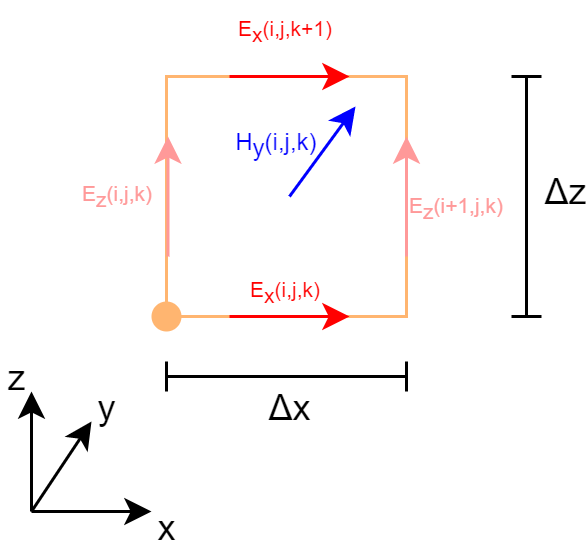
\includegraphics[scale=0.5]{Figures/fdtd3dHyCurl}
	\decoRule
	\caption[3D $H_y$ vector curl]{The curl around the magnetic field vector $H_y$.}
	\label{fig:fdtd3dHyCurl}
\end{figure}

We see that the magnetic vector $H_y(i,j,k)$ is affected by the electric vectors $E_x(i,j,k), E_x(i,j,k+1), E_z(i,j,k)$, and $E_z(i+1,j,k)$. The resulting update equation will then be:
\begin{multline}
	\label{eqn:3dHyCurlFinal}
	H_y^{new}(i,j,k) =  H_y^{prev}(i,j,k) + \frac{\Delta t}{\mu \cdot \Delta s} \cdot \\ (E_z(i+1,j,k) - E_z(i,j,k) - E_x(i,j,k+1) + E_x(i,j,k))
\end{multline}

Before continuing with the magnetic field, let's quickly take a look at the electric vector $E_z$ curl (Figure \ref{fig:fdtd3dEzCurl}). The reasons for this will become apparent shortly.

\begin{figure}[h!]
	\centering
	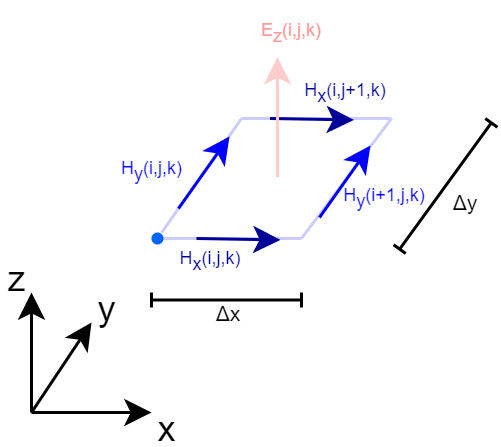
\includegraphics[scale=0.5]{Figures/fdtd3dEzCurl}
	\decoRule
	\caption[3D $E_z$ vector curl]{The curl around the electric field vector $E_z$.}
	\label{fig:fdtd3dEzCurl}
\end{figure}

Again, as we did in the previous chapter the methodology is the same. We must however now account for not only the added dimension, but also the fact that previously one of our magnetic vectors was zero.
Starting off from the initial Maxwell equation:

\begin{equation}
	\label{eqn:magneticIntegral}
	\oint H \cdot ds = \frac{d}{dt} \iint \epsilon \cdot E \cdot dA
\end{equation}
\begin{multline}
	\label{eqn:3dEzCurl1}
	\Rightarrow H_x(i,j-1,k) \cdot \Delta x + H_y(i,j-1,k) \cdot \Delta y - H_x(i,j-1,k) \cdot \Delta x - H_y(i,j-1,k) \cdot \Delta y =\\ \epsilon \cdot \frac{d}{dt} E_z(i,j,k) \cdot \Delta x \cdot \Delta z
\end{multline}

Again taking into account the uniform mesh:
\begin{equation}
	\label{eqn:3dEzCurl2}
	\frac{d E_z(i,j,k)}{dt} = \frac{1}{\epsilon \Delta s} (H_x(i,j-1,k) + H_y(i,j-1,k) - H_x(i,j-1,k) - H_y(i,j-1,k))
\end{equation}

On the left hand side:
\begin{equation}
	\label{eqn:3dEzCurl3}
	\frac{d E_z(i,j,k)}{dt} = \frac{E_z^{new}(i,j,k) - E_z^{prev}(i,j,k)}{\Delta t}
\end{equation}

Finally, by combining equation \ref{eqn:3dEzCurl2} and \ref{eqn:3dEzCurl3}:
\begin{multline}
	\label{eqn:3dEzCurlFinal}
	E_z^{new}(i,j,k) =  E_z^{prev}(i,j,k) + \frac{\Delta t}{\epsilon \cdot \Delta s} \cdot \\ (H_x(i-1,j,k) - H_x(i,j,k) - H_y(i,j,k-1) + H_y(i,j,k))
\end{multline}

We could proceed to manually do the curls for the remaining field vectors, however with a keen eye we can spot a pattern in the equations above, which is shown in formula \ref{eqn:3dCurlPattern}.
\begin{multline}
	\label{eqn:3dCurlPattern}
	V_{a_1}^{new}(i,j,k) =  V_{a_1}^{prev}(i,j,k) + \frac{\Delta t}{\alpha \cdot \Delta s} \cdot \\ (T_{a_2}(C_1) - T_{a_2}(i,j,k) - T_{a_3}(C_2) + T_{a_3}(i,j,k))
\end{multline}

where:

\begin{itemize}
	\item \textbf{V} is the vector field type, which can be either \textbf{E} or \textbf{H}
	\item \textbf{T} is the opposite of \textbf{V}, meaning if $V = E$, then $T = H$
	\item $\boldsymbol{a_1,a_2,a_3}$ symbolize the axes, which need to follow a specific order: $x,y,z,x,y,z,x...$ . As an example, if we have $a_1 = y$, then $a_2 = z$ and $a_3 = x$
	\item $\boldsymbol{\alpha}$ is either $\epsilon$ when calculating for an electric field vector, or $\mu$ for a magnetic one.
	\item $\boldsymbol{C_1, C_2}$ are the indexes of the vectors that are shifted by one in the direction of an axis, which depend on two things: which axis the vector is parallel to, and whether we are calculating for an electric field or a magnetic one.
\end{itemize}

The last point deserves a deeper explanation in order to be elaborated properly. $C_1$ and $C_2$ are indexes of type (i,j,k), where one of the indexes is $\pm1$. If we are calculating the equation for the electric curl, the sign will be $+$. Otherwise it will be $-$. The updated index, meaning the one that will have the $\pm1$, will be the index that does not belong to either the vector we are trying to figure out the equation for, or the vector to which the curl belongs to.

Let us use the $H_x$ vector curl, shown in Figure \ref{fig:fdtd3dHxCurl}, to test our pattern.

\begin{figure}[h!]
	\centering
	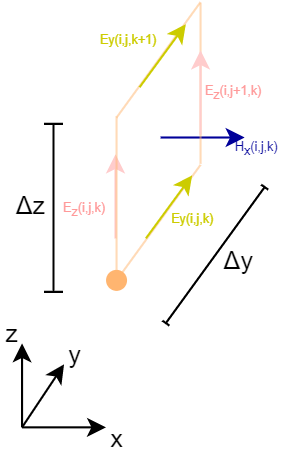
\includegraphics[scale=0.6]{Figures/fdtd3dHxCurl}
	\decoRule
	\caption[3D $H_x$ vector curl]{The curl around the magnetic field vector $H_x$.}
	\label{fig:fdtd3dHxCurl}
\end{figure}

We have the following:

\begin{enumerate}
	\item $V = H$
	\item $T = E$
	\item $a_1 = x$, meaning $a_2 = y$ and $a_3 = z$
	\item $\alpha = \mu$
	\item $C_1$ in this case are the indexes for $E_y$. Since we are doing the curl for $H_x$, that means we are adding one to the $z$ index, meaning that we need to replace $C_1$ with $i,j,k+1$
	\item Similarly, $C_2$ would be replaced by $i,j+1,k$\\
\end{enumerate}

The resulting equation would then be:
\begin{multline}
	\label{eqn:3dHxPatternFinal}
	H_x^{new}(i,j,k) =  H_x^{prev}(i,j,k) + \frac{\Delta t}{\mu \cdot \Delta s} \cdot \\ (E_y(i,j,k+1) - E_y(i,j,k) - E_z(i,j+1,k) + E_z(i,j,k))
\end{multline}

To confirm that the equation is the same, after doing the curls we would get:
\begin{multline}
	\label{eqn:3dHxCurl1}
	H_x^{new}(i,j,k) =  H_x^{prev}(i,j,k) - \frac{\Delta t}{\mu \cdot \Delta s} \cdot \\ (E_y(i,j,k) + E_z(i,j,k) - E_y(i,j,k+1) - E_z(i,j,k))
\end{multline}

On the right hand side, we can flip the $-$ sign on the second half by multiplying the curl in the brackets by $-1$:
\begin{multline}
	\label{eqn:3dHxCurl2}
	H_x^{new}(i,j,k) =  H_x^{prev}(i,j,k) + \frac{\Delta t}{\mu \cdot \Delta s} \cdot \\ -1 \cdot (E_y(i,j,k) + E_z(i,j,k) - E_y(i,j,k+1) - E_z(i,j,k))
\end{multline}

Now, by working only with the curl part, we have:
\begin{multline}
	-1 \cdot (E_y(i,j,k) + E_z(i,j,k) - E_y(i,j,k+1) - E_z(i,j,k)) \\
	\Leftrightarrow (- E_y(i,j,k) - E_z(i,j,k) + E_y(i,j,k+1) + E_z(i,j,k)) \\
	\Leftrightarrow (E_y(i,j,k+1) - E_y(i,j,k) - E_z(i,j+1,k) + E_z(i,j,k))
\end{multline}

Therefore, our final equation is:
\begin{multline}
	\label{eqn:3dHxCurlFinal}
	H_x^{new}(i,j,k) =  H_x^{prev}(i,j,k) + \frac{\Delta t}{\mu \cdot \Delta s} \cdot \\ (E_y(i,j,k+1) - E_y(i,j,k) - E_z(i,j+1,k) + E_z(i,j,k))
\end{multline}

which is equal to equation \ref{eqn:3dHxPatternFinal}.

By using either method, we can derive the update equations for the vectors we have not done yet: $E_x$ (\ref{eqn:3dExCurlFinal}) and $E_y$ (\ref{eqn:3dEyCurlFinal}).
\begin{multline}
	\label{eqn:3dExCurlFinal}
	E_x^{new}(i,j,k) =  E_x^{prev}(i,j,k) + \frac{\Delta t}{\mu \cdot \Delta s} \cdot \\ (H_y(i,j,k-1) - H_y(i,j,k) - H_z(i,j-1,k) + H_z(i,j,k))
\end{multline}
\begin{multline}
	\label{eqn:3dEyCurlFinal}
	E_y^{new}(i,j,k) =  E_y^{prev}(i,j,k) + \frac{\Delta t}{\mu \cdot \Delta s} \cdot \\ (H_z(i-1,j,k) - H_z(i,j,k) - H_x(i,j,k-1) + H_x(i,j,k))
\end{multline}

We can now move on to the implementation.

%----------------------------------------------------------------------------------------
%	SECTION 2
%----------------------------------------------------------------------------------------

\section{C++ Implementation}

Compared to the two-dimensional implementation, we do not have to make too many changes in order to adapt our program for three dimensions. If we use the previous code as a basis, then we already have the packages we need as well as the basic code structure. We can immediately take a look at which environment variables will need changing.

\begin{minted}[breaklines,frame=single,fontsize=\footnotesize]{c++}
int N = 50;
int iterNum = 200;
\end{minted}

It is highly recommended to drastically reduce the size of the domain as well as the number of iterations. The reason is that not only have we increased the amount of update loops from $N^2$ to $N^3$, but we also have six three-dimensional vectors instead of three two-dimensional ones. It is recommended to start from a small number and go up for there. The hardware that we have available can handle around this much, so we will keep these values for now. It is a good thing to note that the resulting files can be too big for Paraview to handle, so that is another limitation there.

We also need to update our \textit{deltaT} equation now that we have three dimensions:

\begin{minted}[breaklines,frame=single,fontsize=\footnotesize]{c++}
double deltaT = (deltaZ * sqrt(permitivity*permeability)  * (1/sqrt(3)));
\end{minted}

Also, we need six three-dimensional vectors for our electric and magnetic fields, all initialized with N zeros in each entry:

\begin{minted}[breaklines,frame=single,fontsize=\footnotesize]{c++}
vector<vector<vector<double>>> Ex(N, vector<vector<double>>(N, vector<double>(N, 0)));
vector<vector<vector<double>>> Ey(N, vector<vector<double>>(N, vector<double>(N, 0)));
vector<vector<vector<double>>> Ez(N, vector<vector<double>>(N, vector<double>(N, 0)));
vector<vector<vector<double>>> Hx(N, vector<vector<double>>(N, vector<double>(N, 0)));
vector<vector<vector<double>>> Hy(N, vector<vector<double>>(N, vector<double>(N, 0)));
vector<vector<vector<double>>> Hz(N, vector<vector<double>>(N, vector<double>(N, 0)));
\end{minted}

Next we need to modify the functions that create CSV files or our data. Now that we have an equal number of vectors for both the electric and the magnetic wave, we only need one function that handles both vectors:

\begin{minted}[breaklines,frame=single,fontsize=\footnotesize]{c++}
void writeDataToCsvFile(string filename, vector<vector<vector<double>>> Vx, vector<vector<vector<double>>> Vy, vector<vector<vector<double>>> Vz){
	
	//	x,y,z,Vx,Vy,Vz
	//	0,0,Vx[x,y,z],Vy[x,y,z],Vz[x,y,z]
	
	ofstream csvFile(filename);
	csvFile << "x,y,z,Vx,Vy,Vz\n";
	
	for (unsigned  x = 0; x < Vx[0][0].size(); x++) {
		for (unsigned  y = 0; y < Vy[x][0].size(); y++) {
			for (unsigned  z = 0; z < Vz[x][y].size(); z++) {
				csvFile << x << "," << y << "," << z << "," << Vx[x][y][z] << "," << Vy[x][y][z] << "," << Vz[x][y][z] << "\n";
			}
		}
	}
	
	csvFile.close();
}
\end{minted}

For our main loop, we can apply the Gaussian Pulse excitation to either an electric field vector or the magnetic one. Both work, but we need to keep in mind that when using the magnetic field for the excitation, we need to lower the magnitude if using vacuum as a medium. Depending on the material used in the domain, this may be unnecessary. Again, we apply this excitation in the middle of our vector so that we have a nice symmetrical wave propagation.

\begin{minted}[breaklines,frame=single,fontsize=\footnotesize]{c++}
Ex[24][24][24] = exp(-(beta * pow((t - gamma), 2)));
\end{minted}

We only need one vector, and this will also affect the order of our update loops. If using an electric vector for the excitation, the loop order is as follows:

\begin{minted}[breaklines,frame=single,fontsize=\footnotesize]{c++}
// loop for values
for (int i = 0; i < N-1; i++) {
	for (int j = 0; j < N-2; j++) {
		for (int k = 0; k < N-2; k++) {
			Hx[i][j][k] = Hx[i][j][k] + (deltaT / permeability / deltaZ) * (Ey[i][j][k+1] - Ey[i][j][k] - Ez[i][j+1][k] + Ez[i][j][k]);
		}
	}
}

for (int i = 0; i < N-2; i++) {
	for (int j = 0; j < N-1; j++) {
		for (int k = 0; k < N-2; k++) {
			Hy[i][j][k] = Hy[i][j][k] + (deltaT / permeability / deltaZ) * (Ez[i+1][j][k] - Ez[i][j][k] - Ex[i][j][k+1] + Ex[i][j][k]);
		}
	}
}

for (int i = 0; i < N-2; i++) {
	for (int j = 0; j < N-2; j++) {
		for (int k = 0; k < N-1; k++) {
			Hz[i][j][k] = Hz[i][j][k] + (deltaT / permeability / deltaZ) * (Ex[i][j+1][k] - Ex[i][j][k] - Ey[i+1][j][k] + Ey[i][j][k]);
		}
	}
}

writeDataToCsvFile((filePath + "H/H.csv." + to_string(i)), Hx, Hy, Hz);

for (int i = 0; i < N-1; i++) {
	for (int j = 1; j < N-1; j++) {
		for (int k = 1; k < N-1; k++) {
			Ex[i][j][k] = Ex[i][j][k] + (deltaT / permitivity / deltaZ) * (Hy[i][j][k-1] - Hy[i][j][k] - Hz[i][j-1][k] + Hz[i][j][k] );
		}
	}
}

for (int i = 1; i < N-1; i++) {
	for (int j = 0; j < N-1; j++) {
		for (int k = 1; k < N-1; k++) {
			Ey[i][j][k] = Ey[i][j][k] + (deltaT / permitivity / deltaZ) * (Hz[i-1][j][k] - Hz[i][j][k] - Hx[i][j][k-1] + Hx[i][j][k]);
		}
	}
}

for (int i = 1; i < N-1; i++) {
	for (int j = 1; j < N-1; j++) {
		for (int k = 0; k < N-1; k++) {
			Ez[i][j][k] = Ez[i][j][k] + (deltaT / permitivity / deltaZ) * (Hx[i][j-1][k] - Hx[i][j][k] - Hy[i-1][j][k] + Hy[i][j][k]);
		}
	}
}

writeDataToCsvFile((filePath + "E/E.csv." + to_string(i)), Ex, Ey, Ez);

}
\end{minted}

When using a magnetic vector for the excitation, we would need to run the electric loops first. And again, we need to keep in mind that our loop indexes do not go out of bounds for the magnetic field equations.

With that said, after running the program we should have 200 files (indexed from 0 to 199) that we can grab and place in Paraview as we did before.

\section{Data Visualization}

The process for three-dimensional data is going to be almost exactly the same as the two-dimensional scenario in the previous chapter. The main caveat here is to make sure to update the equation for the \textbf{Calculator} filter by clicking it in the \textbf{Pipeline Browser} and on the properties page type \mint{c++}{iHat*Vx+jHat*Vy+kHat*Vz}. Please note that Vx,Vy, and Vz, are taken directly from the header of our CSV files. If that header is different, we need to reflect that here. In our case, we are using \textit{"x,y,z,Vx,Vy,Vz"}.

After setting it up and playing around with the configurations a bit, we can get the following simulation for our electric data (Figure \ref{fig:FDTD3DE}).

\begin{figure}[h!]
	\centering
	\begin{subfigure}{.49\textwidth}
		\centering
		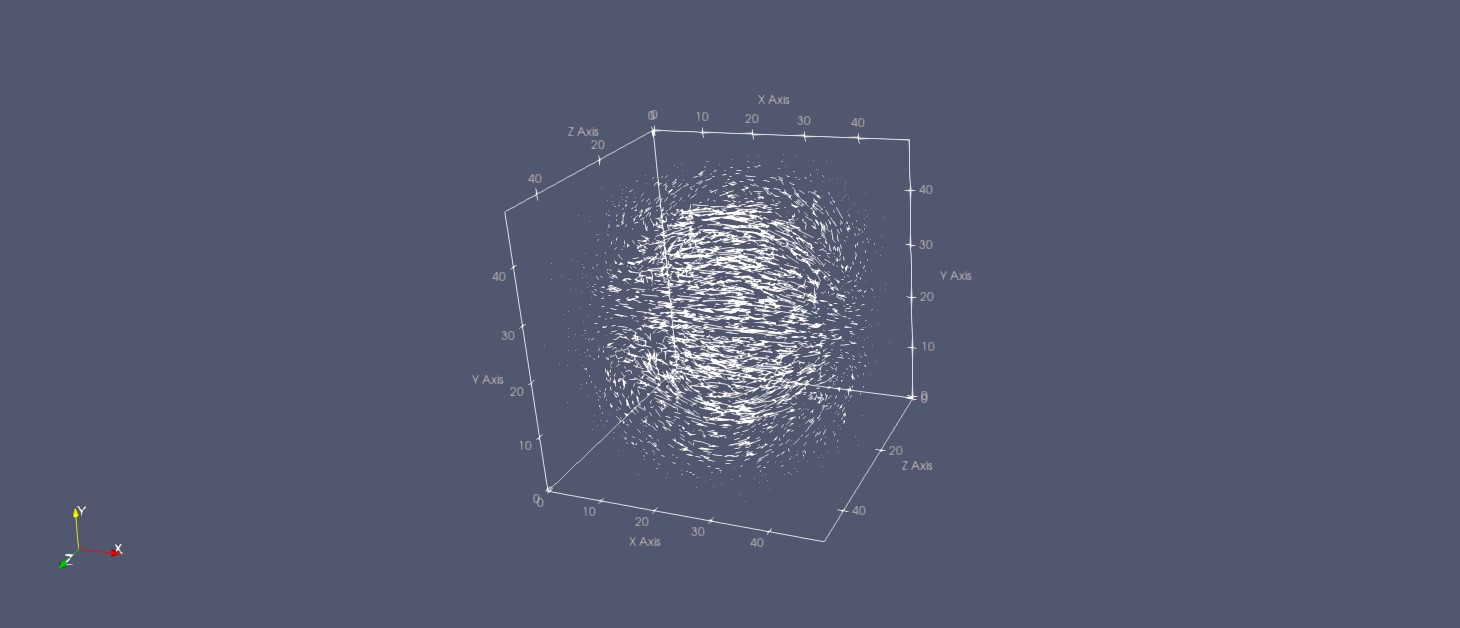
\includegraphics[width=.95\linewidth]{Figures/FDTD3DE1}
		\caption{t = 50}
	\end{subfigure}
	\begin{subfigure}{.49\textwidth}
		\centering
		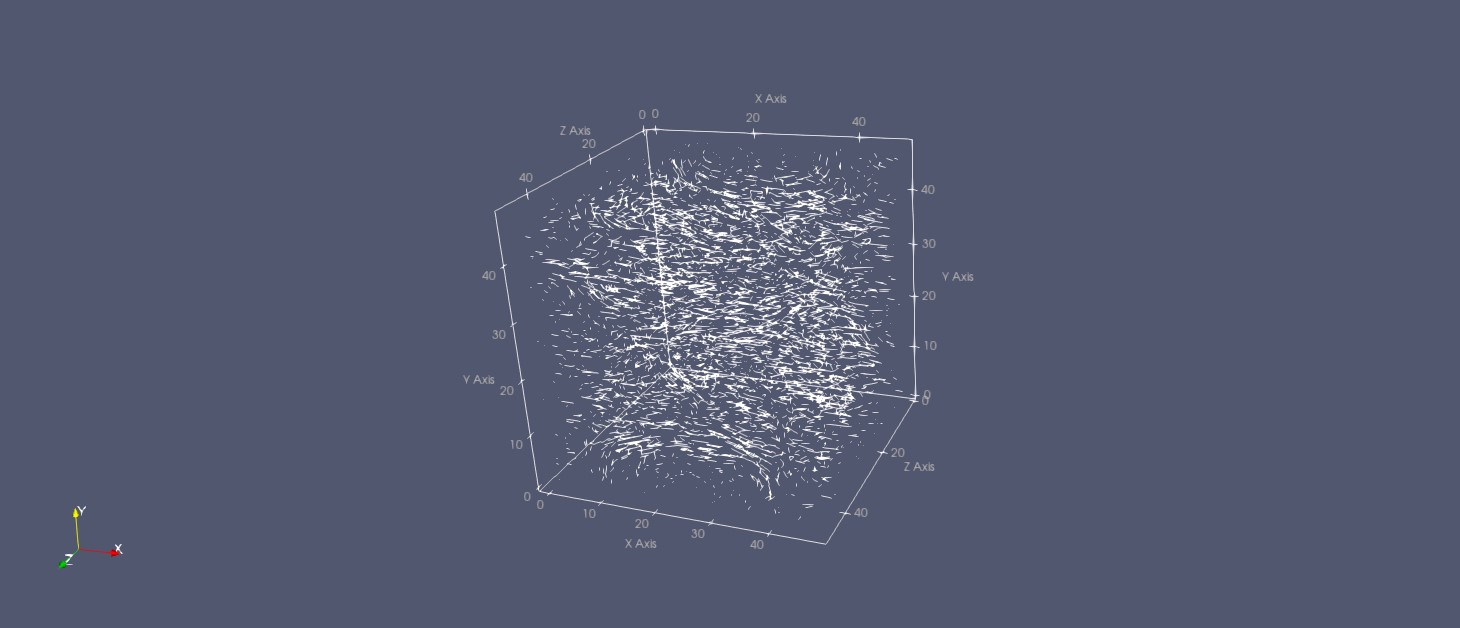
\includegraphics[width=.95\linewidth]{Figures/FDTD3DE2}
		\caption{t = 100}
	\end{subfigure}
	\begin{subfigure}{.49\textwidth}
		\centering
		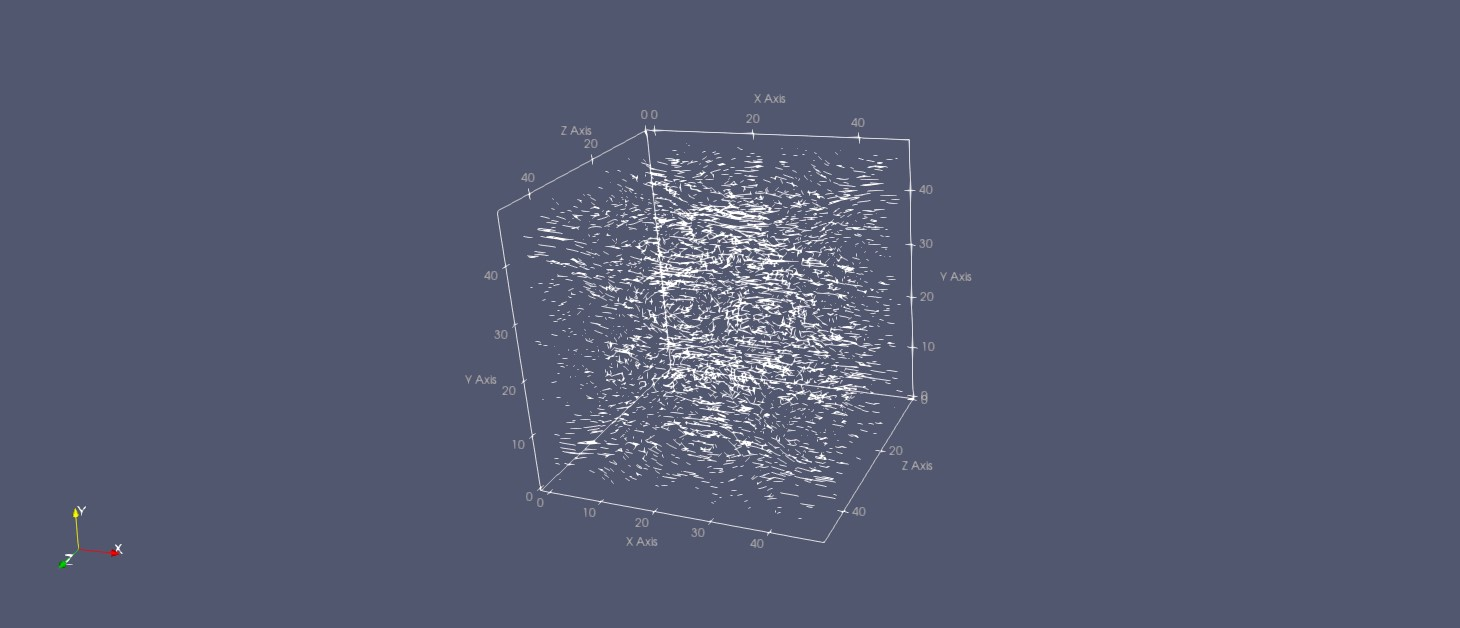
\includegraphics[width=.95\linewidth]{Figures/FDTD3DE3}
		\caption{t = 150}
	\end{subfigure}
	\begin{subfigure}{.49\textwidth}
		\centering
		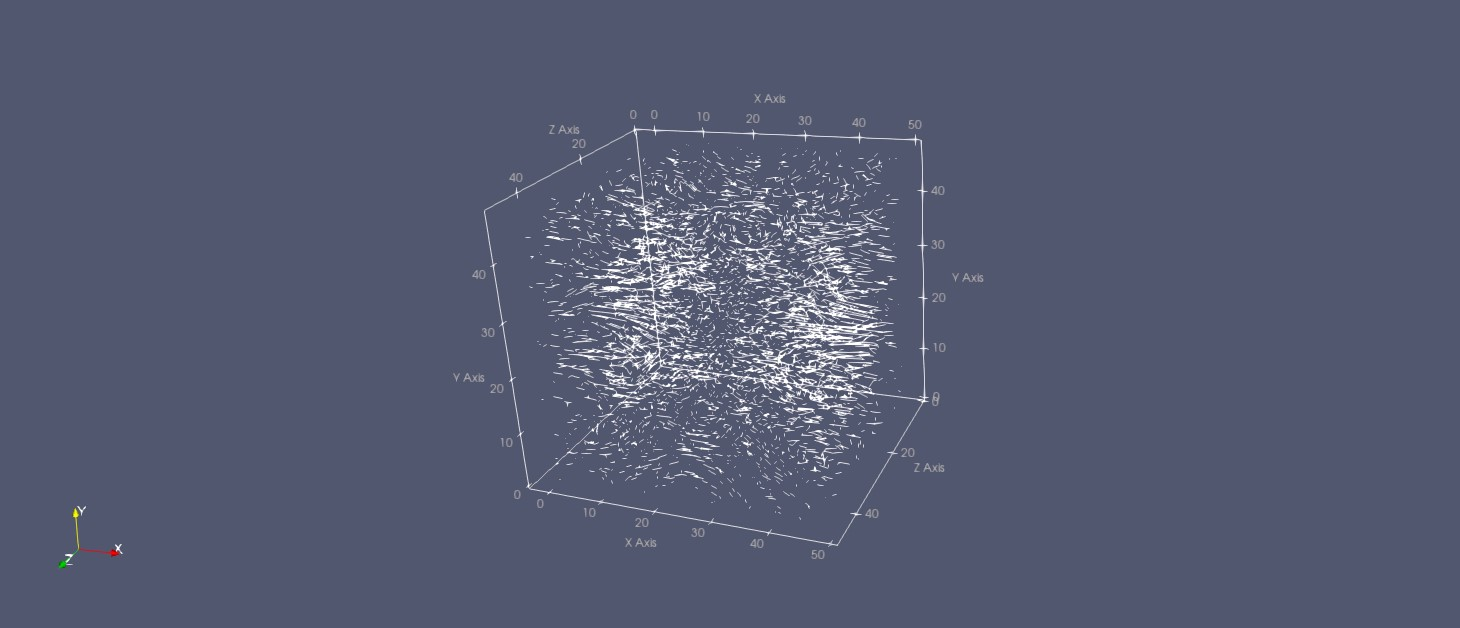
\includegraphics[width=.95\linewidth]{Figures/FDTD3DE4}
		\caption{t = 200}
	\end{subfigure}
	\decoRule
	\caption[3D Electric Field Simulation]{A simulation of the 3D electric field.}
	\label{fig:FDTD3DE}
\end{figure}

Following the same steps, we can do the same for the magnetic data as well. Please note that we scale this data up a bit, as it would be quite hard to see otherwise due to using vacuum as a medium.

\begin{figure}[h!]
	\centering
	\begin{subfigure}{.49\textwidth}
		\centering
		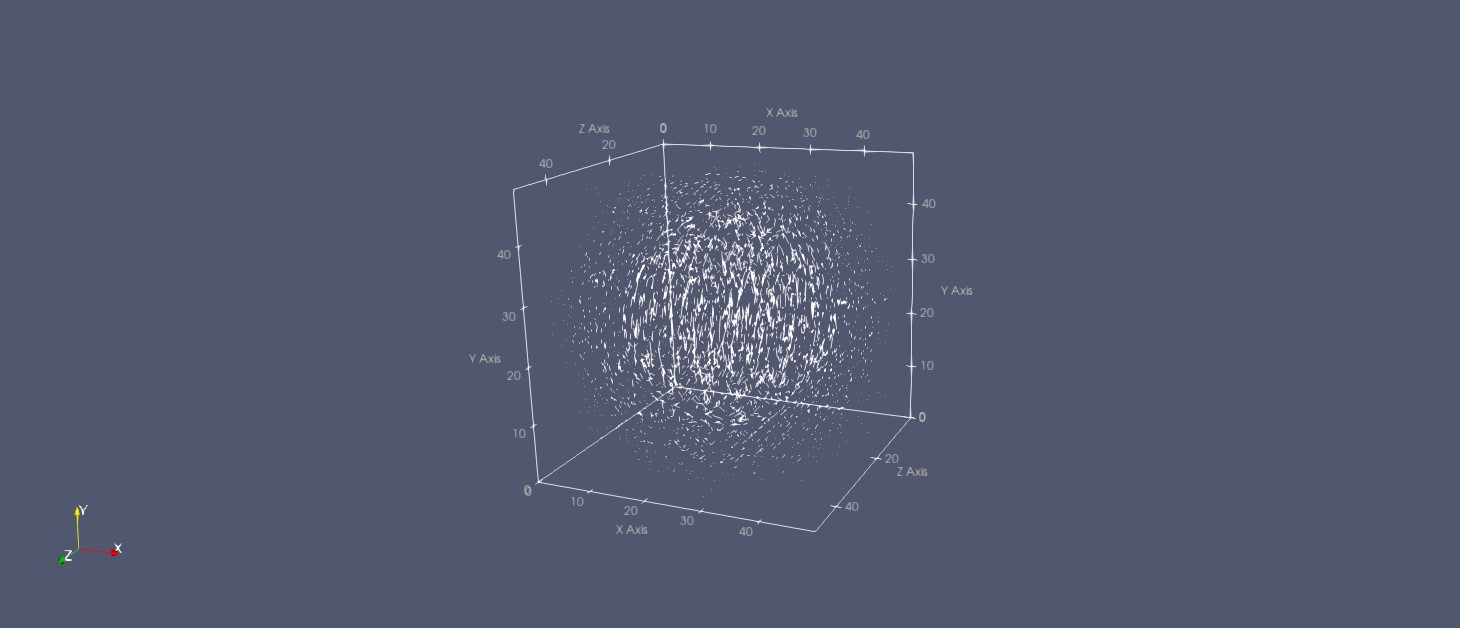
\includegraphics[width=.95\linewidth]{Figures/FDTD3DH1}
		\caption{t = 200}
	\end{subfigure}
	\begin{subfigure}{.49\textwidth}
		\centering
		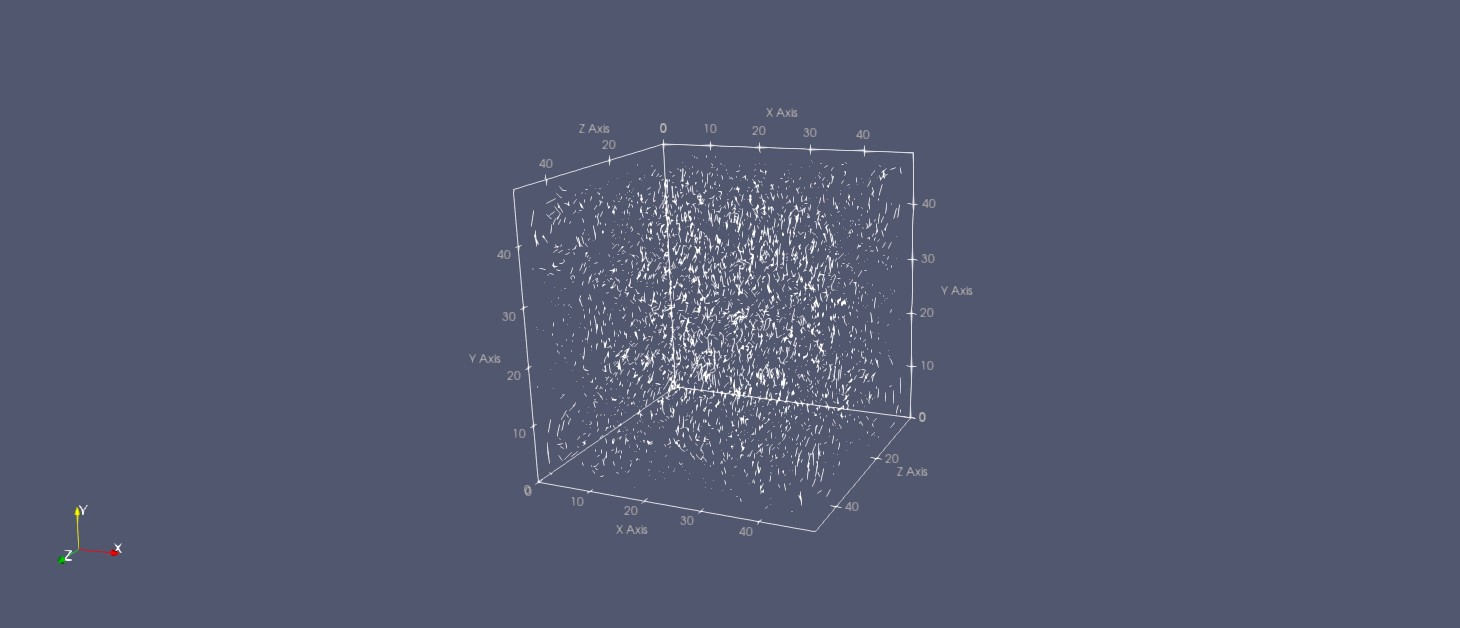
\includegraphics[width=.95\linewidth]{Figures/FDTD3DH2}
		\caption{t = 400}
	\end{subfigure}
	\begin{subfigure}{.49\textwidth}
		\centering
		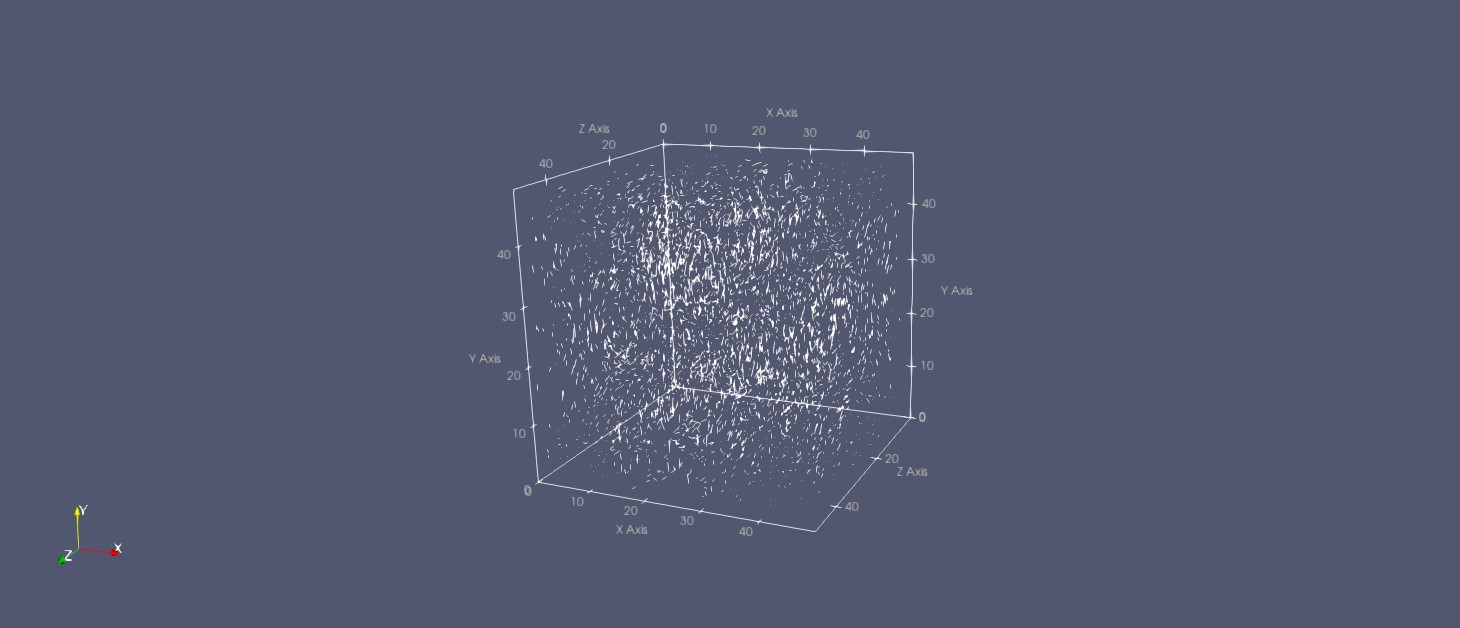
\includegraphics[width=.95\linewidth]{Figures/FDTD3DH3}
		\caption{t = 600}
	\end{subfigure}
	\begin{subfigure}{.49\textwidth}
		\centering
		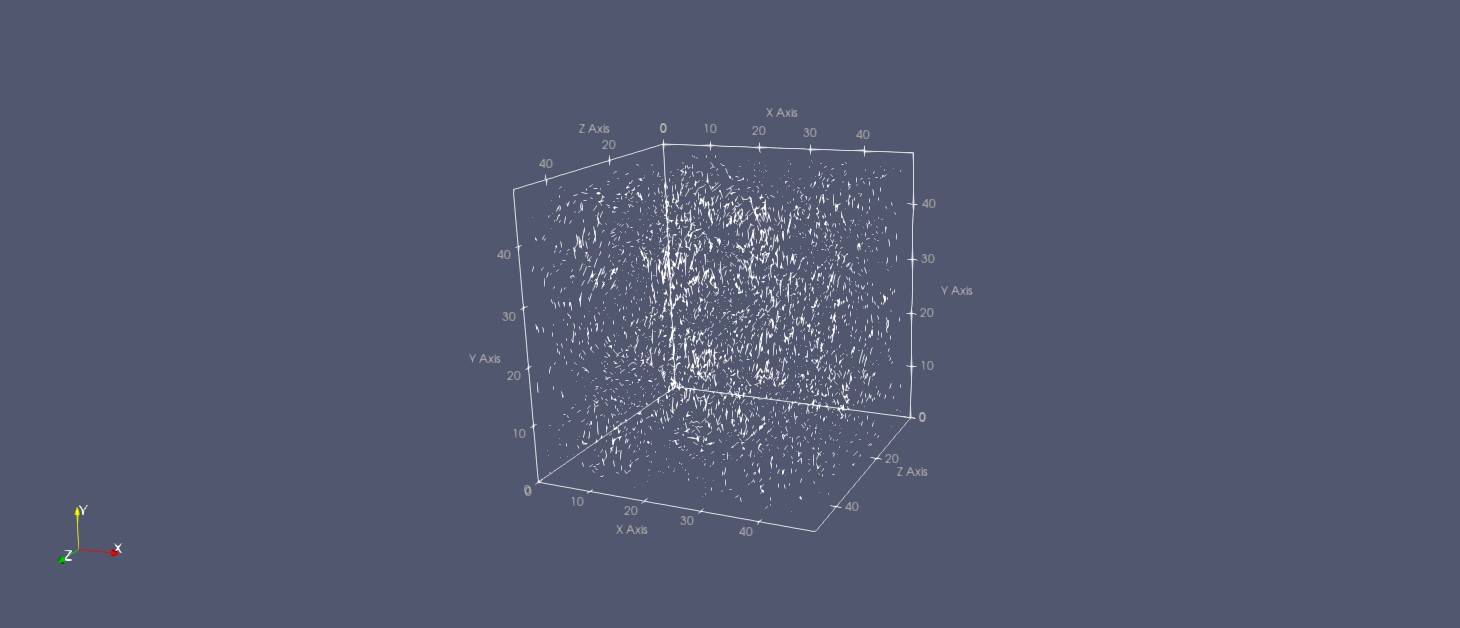
\includegraphics[width=.95\linewidth]{Figures/FDTD3DH4}
		\caption{t = 800}
	\end{subfigure}
	\decoRule
	\caption[3D Magnetic Field Simulation]{A simulation of the 3D magnetic field.}
	\label{fig:FDTD3DH}
\end{figure}

And with that, we have completed our simulation for a three-dimensional scenario. 